\section{Why does EnergyPlus exist and what were its original goals?}\label{why-does-energyplus-exist-and-what-were-its-original-goals}

The existence of EnergyPlus is directly related to some of the increasingly obvious shortcomings of its predecessor programs---BLAST and DOE--2. Both programs, though still valid tools that will continue to have utility in various environments, have begun to show their age in a variety of ways. Both BLAST and DOE--2 were written in older version of FORTRAN and used features that will eventually be obsolete in new compilers. Both programs consisted of a significant amount of ``spaghetti code'' and outdated structures that made it difficult to maintain, support, and enhance. Neither BLAST nor DOE--2 is able to correctly handle feedback from the HVAC system to the zone conditions.

Finally, the speed with which new technology in the HVAC field is developed has far outpaced the ability of the support and development groups of both programs to keep the programs current and viable. This is really the key issue in the existence of EnergyPlus: there simply are not enough researchers worldwide who have enough experience with the complex code of the programs to keep pace with new technology. In addition, due to the years of experience necessary to make modifications to either BLAST or DOE--2, it is extremely expensive and time consuming to produce models or train someone to become proficient in either program's code. The following paragraphs address how the goals of EnergyPlus have been carefully selected to solve the problems of the legacy programs and to make EnergyPlus an international repository for algorithms that can be made available to all interested parties.

\textbf{\emph{Structure and Simulation Management:}} The ``spaghetti code'' nature of the parent programs resulted in great confusion as to how information flowed within the program, when data was modified or should be modified, and what was happening when. Thus, one of the goals of EnergyPlus development was to eliminate the interconnections between various program sections and the need to understand all parts of the code just to make an addition to a very limited part of the program. This goal was achieved through a program structure that implemented a ``manager'' philosophy. In effect, the program consists of many pieces (i.e., modules---see next paragraph) which when viewed graphically resemble an inverted tree. Instead of allowing lower level pieces of the program and calls to those sections of the code to infiltrate up to the highest level of the simulation, each branch exercises control over when its sub-branches are called. Thus, this is much like an organization chart where management over employees proceeds up a chain of command until it reaches the ``CEO'' of the simulation. In EnergyPlus, a subroutine called ManageSimulation serves the ``CEO'' role. This single subroutine controls four of the five main simulation loops (environment, day, hour, sub-hour time step; the system time step is controlled by the HVAC manager). In addition, this subroutine also sets global flags that are used by other subroutines and modules to determine the state of the simulation so that each part of the program knows whether to read input, initialize, simulate, report, etc. The manager philosophy makes the links between program modules simple and explicit. Typically, each module is accessible only through a call to its manager routine. Developers no longer have to worry about hidden and unexpected connections between and among program subroutines.

\textbf{\emph{Modularity:}} One of the benefits of the structural improvements over the legacy programs is that the code can now be much more object-oriented and modular in nature. A result of the goal for improved structure in EnergyPlus was the definition of a well-organized, module concept that would facilitate adding features and links to other programs. It was decided that FORTRAN90 would be used for the initial release of EnergyPlus due to the fact that it:

\begin{itemize}
\item
  is a modern, modular language with good compilers on many platforms
\item
  allows C-like data structures and mixed language modules
\item
  provides structure that begins to be object-based
\item
  allows long variable names (up to 32 characters)
\item
  provides backward compatibility with legacy code during the development process
\end{itemize}

The key benefit of modularity is that researchers can develop modules concurrently without interfering with other modules under development and with only a limited knowledge of the entire program structure. This feature is critical to promoting both widespread use and broad development of program models. EnergyPlus can only be successful if the pool of potential model developers increases significantly so that interest and economics drives what models are added to the program rather than have its extensions limited by a lack of intellectual resources. Thus, modularity and structure improvements in EnergyPlus solve the problems of not having enough experts to keep up with technology and the large start-up time and expense previously needed to bring someone up to speed on program additions.

Since the original version (2001), EnergyPlus code and structure continued to evolve and adopt the ever changing Fortran Standard. However, in 2014, a full conversion of the simulation code to C++ was completed. The development team also adapted workflows and open sourced the code and posted it on \href{https://github.com/NREL/EnergyPlus}{Github}. Just like how the Fortran simulation code utilized modern Fortran standard capabilities, the C++ code utilizes modern (C++11\ldots{}) C++ standard capabilities.

\textbf{\emph{Established Links:}} The modularity of EnergyPlus makes it easier for other developers to quickly add other component simulation modules. This means that it will be significantly easier to establish links to other programming elements. Since initially the EnergyPlus code will contain a significant number of existing modules, there will be many places within the HVAC code where natural links to new programming elements can be established. These are fully documented to assist other developers in a swift integration of their research into EnergyPlus. In addition to these more natural links in the HVAC section of the code, EnergyPlus will also have other more fluid links in areas such as the heat balance that will allow for interaction where the modules might be more complex or less component based. Again, the goal of this feature of EnergyPlus is maximize the number of developers who can quickly integrate their work into EnergyPlus for the minimum investment of resources. The following diagram depicts how other programs have already been linked to EnergyPlus and a big picture view of how future work can impact the program.

\begin{figure}[hbtp] % fig 1
\centering
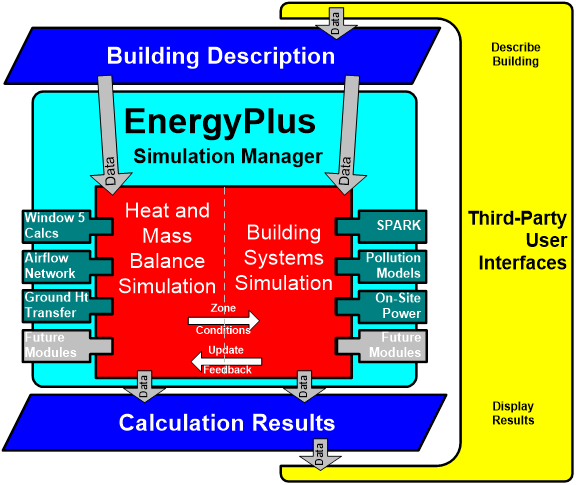
\includegraphics[width=0.9\textwidth, height=0.9\textheight, keepaspectratio=true]{media/image001.png}
\caption{EnergyPlus -- the big picture \protect \label{fig:energyplus-the-big-picture}}
\end{figure}

\textbf{\emph{Integration of Loads, Systems, and Plants:}} One of the strong points of EnergyPlus is the integration of all aspects of the simulation---loads, systems, and plants. Based on a research version of the BLAST program called IBLAST, system and plant output is allowed to directly impact the building thermal response rather than calculating all loads first, then simulating systems and plants. The simulation is coupled allowing the designer to more accurately investigate the effect of undersizing fans and equipment and what impact that might have on the thermal comfort of occupants within the building. The diagram below shows a basic overview of the integration of these important elements of a building energy simulation.

\begin{figure}[hbtp] % fig 2
\centering
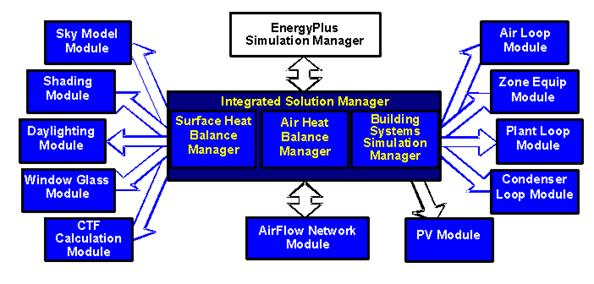
\includegraphics[width=0.9\textwidth, height=0.9\textheight, keepaspectratio=true]{media/image002.jpg}
\caption{EnergyPlus -- Internal elements \protect \label{fig:energyplus-internal-elements}}
\end{figure}

\textbf{\emph{``Open'' Source Code:}} Another advantage of EnergyPlus that it shares with both BLAST and DOE--2 is that the source code of the program will be available and open for public inspection, revision, etc. The program is not intended to be a black box that is unintelligible to the users and developers around the world. While there are many conflicting ideas on what is meant by ``open'', EnergyPlus is certainly not closed since this would be counter to the goals that have already been stated. The hope is that this access to source code will improve the accuracy and usability of the program over the long term and allow many developers to work on the program simultaneously. This ``developer friendly'' stance is critical to keeping EnergyPlus current and in step with technological advances.

In summary, the goals of EnergyPlus are ambitious but achievable via the path described above. EnergyPlus aims to be a program that is relatively simple to work with from the perspective of both the users and the developer. The development team made tremendous efforts to keep simulation code and algorithms as separate as possible and as modular as possible to minimize the overall knowledge that someone would need to have to add models to the program. This will minimize the resource investment and maximize the impact of current research in the field of building energy analysis and thermal load calculations. Finally, the full coupling of building envelopes, systems, and plants will provide a better understanding of how a building responds not only to the environmental factors that impact the building but also the HVAC system as it attempts to meet the thermal loads on the building.

It is also important to note that testing and verification are key issues in the development of any new program such as EnergyPlus. While there are large sections of EnergyPlus that consist of brand new code, the majority of the heat balance code can be traced back to the original parent programs. It should be noted that while this code has been significantly reengineered the team used what has been termed an ``evolutionary reengineering'' (ER) process. In ER, program code is modified stepwise in an effort to restructure it, modularize it, replace old obsolete data structures, etc. The ultimate goal is to bring it up to current programming standards without starting over with new code. At each step along the way, the program is exercised over a variety of input files and parameters to insure that what were intended to be algorithm neutral changes in the program have not resulted in changes to the output. This process was very successful and bolstered confidence in the program. In addition, comparisons could be made back to legacy programs to show that the new program is at a minimum as accurate as its predecessors. Beyond this, EnergyPlus has also been subjected to a lengthy and rigorous testing plan by an outside agency as well as numerous beta testers. This level of effort and collaboration is unprecedented in the history of energy analysis and thermal load calculation programs and has resulted in a much higher level of confidence in the results produced by EnergyPlus.
